\documentclass[a4paper,12pt]{article}
\DeclareMathSizes{12}{30}{16}{12}

\usepackage[T1]{fontenc}
\usepackage[utf8]{inputenc}
\usepackage[english]{babel}

\usepackage[margin=3cm]{geometry}
\usepackage{graphicx}
\usepackage{float}
\usepackage{blindtext}
\usepackage{titling}
\usepackage{titlesec}
\usepackage[center]{caption}
\usepackage[symbol]{footmisc}
\usepackage{wrapfig}
\usepackage{animate}
\usepackage{array}
\usepackage{textcomp}
\usepackage{enumitem}
\usepackage{multirow}
\usepackage{url}
\setlist[enumerate]{itemsep=0mm}


\titleformat{\section}
{\Large\bfseries}
% {\Roman{section}.}
{\thesection.}
{0.5em}
{}

\titleformat{\subsection}
{\center\large\bfseries}
% {\Roman{subsection}}
{\thesubsection}
{0.5em}
{}

\titlespacing{\subsection}
{2em}{2.5em}{0.5em}

\title{Využití umělé inteligence a genetického algoritmu pro autonomní řízení}
\author{Marek Bečvář}
\date{Červen 2020}

\renewcommand{\maketitle}
{
    \begin{center}
        \vspace*{0cm}
        \LARGE{\textbf{\thetitle}}\\
        \vspace{0.5cm}
        \Large{\textbf{\theauthor}}\\
        \vspace{0.5cm}
        \normalsize{\thedate}
        \vspace{0.2cm}
        \hrule
    \end{center}
}

\addto\captionsenglish{\renewcommand{\figurename}{Schéma}}
\addto\captionsenglish{\renewcommand{\tablename}{Tabulka}}

\addto\captionsenglish{\renewcommand{\contentsname}{Obsah}}
\addto\captionsenglish{\renewcommand{\listfigurename}{Seznam obrázků}}
\addto\captionsenglish{\renewcommand{\refname}{Seznam literatury}}


\renewcommand{\figurename}{}

\renewcommand{\thefootnote}{\fnsymbol{footnote}}

\newcommand{\tab}
{
    \hspace*{1em}
}

\linespread{1.25}
\begin{document}
    \maketitle

    \vspace{0.25cm}
    \section{O projektu}
        \tab Tento projekt byl zpracován v roce 2020 jako maturitní z předmětu Informatika 
        a výpočetní technika práce v 6.ročníku Gymnázia Boženy Němcové v Hradci Králové.\\
        \tab Hlavní myšlenkou je využití strojového učení umělé inteligence genetickým 
        algoritmem s cílem projetí uživatelem nastavené tratě. Výsledek snažení 
        je postupně promítán do grafu. Schopnost by se měla, i po dosažení cíle (projetí tratí),
        stále rozvíjet.

    \section{Mechanismy programu}
    \subsection{Umělá inteligence}
        Pojem \textbf{umělé inteligence} je dnes člověku prezentován v trochu zkreslené formě.
        Lidem se mohou vybavit některé sci-fi filmové scény s roboty, ale to není úplně přesné.
        Ve slově \textit{inteligence} se doopravdy skrývá řada výpočtů zpracovávajících \\vstupní data 
        na požadovaný výstup. Tyto výpočty se provádějí v předem definované 
        struktuře tzv. \textbf{neuronové sítě}.\\
            
        \begin{figure}[H]
        \centering
        \begin{minipage}[t]{.5\textwidth}
            \centering
            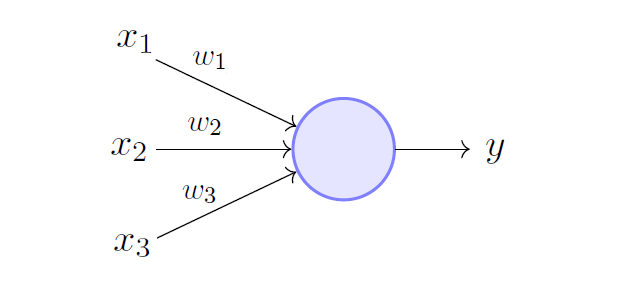
\includegraphics[width=0.9\linewidth]{data/perceptron-model1.png}
            \captionof{figure}{Perceptron \cite{c:perceptron}}
            \label{fig:perceptron}
        \end{minipage}%
        \begin{minipage}[t]{.5\textwidth}
            \centering
            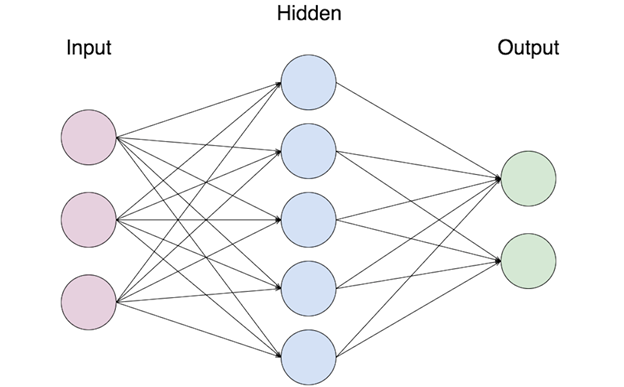
\includegraphics[width=0.85\linewidth]{data/easynn-scheme.png}
            \captionof{figure}{Neuronová síť \cite{c:easynn}}
            \label{fig:easynn}
        \end{minipage}
        \end{figure}

        Neuronová síť je modelována s inspirací v mozkových neuronech. Každý bod je považován za
        samostatný neuron a každý neuron je propojen s řadou dalších (\textit{podobně jako struktura mozku})
        Právě tato spojení jsou důležitou funkční složkou neuronových sítí. V programu tedy vždy 
        uchováváme číselnou hodnotu každého z nich. Tato hodnota je obvykle reálné číslo v rozsahu od -1.0 do 1.0.
        Neurony dělíme do vrstev (VSTUP, SKRYTÁ, VÝSTUP). Data ze sledovaného prostředí přenášíme
        do vstupní vrstvy a výsledek pozoruje na vrstvě výstupní. Existuje pravidlo, že každý neuron z nižší vrstvy,
        je spojen se všemi neurony ve vyšší vrstvě. Nejjednodušším znázorněním neuronu je 
        Schéma~\ref{fig:perceptron}, skládající se z 3 vstupů a 1 výstupu.
        Jak se ale tvoří číselné hodnoty?
        \vspace{-0.05em}
        \begin{equation}
            \sigma(\displaystyle\sum_{k=1}^{n}{x_k * w_k})
        \end{equation}
        \vspace{-0.2cm}
        \begin{equation}
            \scriptscriptstyle 0.5*0.1 + 1.0*0.5 + 0.25*0.3 = 0.625 \hspace*{0.2cm} \rightarrow \hspace*{0.2cm}
            \sigma(0.625)=0.625
        \end{equation}

        kde $\scriptstyle \sigma$ je \textit{aktivační funkce}. Tyto funkce pouze upravují 
        možný rozsah výstupních hodnot. Takto získáme finální hodnotu na jednom neuronu.\\

        \begin{wrapfigure}[5]{r}{0.4\textwidth}
            \vspace{-2.5em}
            \centering
            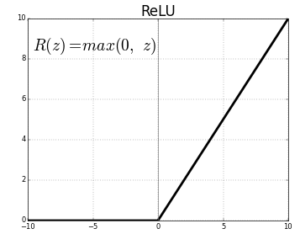
\includegraphics[width=0.8\linewidth]{data/relu.png}
            \caption{RELU aktivační funkce \cite{c:relu}} 
            \label{fig:relu}
        \end{wrapfigure}

        Příkladem takové aktivační funkce může být třeba \textbf{RELU} (Rectified Linear Unit).
        Ta výstupní hodnoty změní tak, že kladné nechá beze změny a záporné změní na nulu.
        Tyto změny pomáhají při přenosu signálu mezi neurony v síti.
        \\\\\\\\
        \begin{flushleft}
            \vspace{-3.1em}
            Složitější neuronové sítě jsou už jen opakováním tohoto zavedeného postupu. Dále se pro sítě 
            tohoto typu zavádí termín \textbf{hluboká neuronová síť} (\textit{z ang. deep neural network}). 
            To označuje schéma, ve kterém je použita více než jedna skrytá vrstva.
        \end{flushleft}

        \vspace{-0.3em}
        \begin{figure}[H]
            \centering
            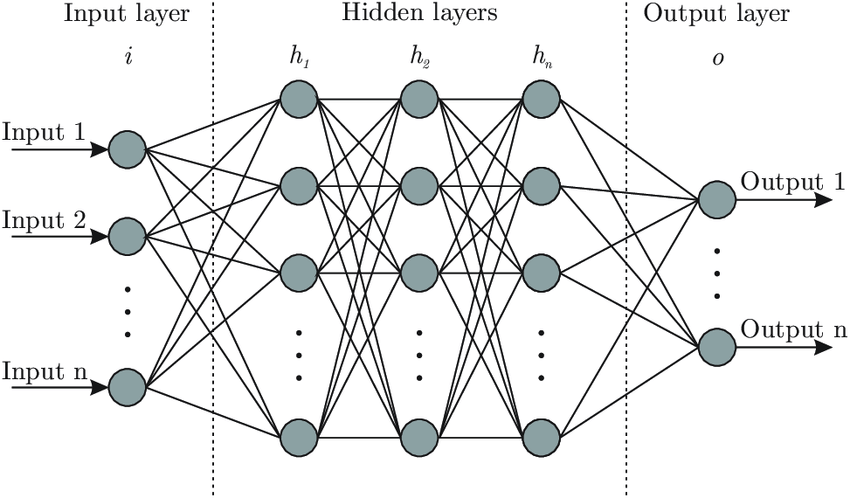
\includegraphics[width=0.51\textwidth]{data/nn-scheme.png}
            \captionof{figure}{Hluboká neuronová síť \cite{c:deepnn}}
            \label{fig:deepnn}
        \end{figure}

        Při práci s neuronovými sítěmi, abychom zvětšili přesnost výpočtů, upravujeme vstupy
        (první řadu neuronů) do určitého číselného rozsahu. Poté necháme proběhnout všechny 
        matematické operace uvnitř sítě a sledujeme výsledek. To, jak se program bude při daném 
        výsledku chovat, je opět pouze na volbě autora programu.\\\\
        \tab Poté nastává \textbf{proces učení}, při kterém upravujeme hodnoty všech spojení v síti tak,
        aby při určitých vstupních hodnotách nastal požadovaný výstup. Pro učení existuje řada algoritmů
        založených na různých matematických úpravách. Pro moji síť jsem ale zvolil postup učení
        inspirovaný přírodou, tzv. \textbf{genetický algoritmus} (\textit{"O původu druhů" Charles Darwin - evoluční teorie}).\\\\
        \tab Samotná architektura (počet neuronů v každé z vrstev) je pro funkčnost velmi
        důležitá a neexistuje předem daný, jednoznačně správný postup. Tato část je tedy často o 
        spoustě drobných úprav při hledání dobře pracující sítě.\\
        \tab Architektura, která je použita v prezentovaném programu, byla docílena řadou testů
        různých sítí proti sobě.\\\\
        \textbf{Finální síť použitá v programu je ve schématu \{6, 8, 4, 2\}}\\
        5 vstupů měřících vzdálenost + 1 vstup měřící čas\\
        1 výstup pro rychlost + 1 výstup pro zatáčení

    \subsection{Genetický algoritmus}
        Genetický algoritmus má v informatice mnoho využití při řešení logických problémů. 
        Ve svém projektu jsem ho použil na úpravu spojů v neuronové síti. Algoritmus je také známý svými 
        procesy, které přímo kopírují fungování v přírodě. Teorie genetického algoritmu je založena 
        na Darwinově teorii (\textit{"O původu druhů"})\\
        \tab Rozlišujeme jedince, jejichž genetickou informací jsou všechny hodnoty spojů v neuronové síti. 
        Při učení procházíme stálým cyklem, při kterém se tato genetická informace upravuje tak, 
        aby se výsledky zlepšovaly.
        \vspace{0.5cm}
        \begin{figure}[H]
            \centering
            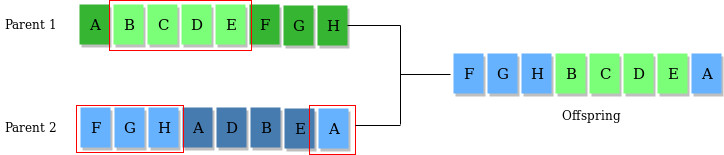
\includegraphics[width=0.8\textwidth]{data/genetic-algorithm.png}
            \captionof{figure}{Genetický crossover \cite{c:crossover}}
            \label{fig:crossover}
        \end{figure}

        \underline{\textbf{\large{Cyklus genetického algoritmu}}}
        \begin{enumerate}[itemsep=-1.5mm] 
            \item Určíme, jak velký počet jedinců chceme testovat (\textbf{velikost populace})
            \item Naplníme populaci náhodně generovanými jedinci.
            \begin{itemize}[noitemsep]
                \item každý jedinec je abstrakcí jedné náhodné neuronové sítě
                \item všechna spojení sítě tvoří genetickou informaci
            \end{itemize}
            \item Všechny jedince v populaci vyzkoušíme v testovacím prostředí a zapíšeme jejich \textbf{zdatnost}
                v zadaném problému.
            \item Z populace pseudo-náhodně vybereme skupinu rodičů nové generace.
            \begin{itemize}[noitemsep]
                \item ti s \textbf{vyšší zdatností mají větší šanči} být zvoleni mezi rodiče
                \item každý z jedinců může být zvolen opakovaně
            \end{itemize}
            \item Ze skupiny rodičů náhodně vybereme vždy dva jedince a náhodným poskládáním jejich
                genetických informací vytvoříme dva nové potomky (\textbf{genetický crossover} Schéma~\ref{fig:crossover}).
            \item Každý gen každého potomka má určitou šanci náhodně zmutovat.
            \begin{itemize}[noitemsep]
                \item hodnotu této náhody musíme určit
                \item \textbf{pravděpodobnost mutace} se obvykle pohybuje mezi 1\% - 5\%\\
                    Příliš malá hodnota a populace není schopna prozkoumávat nová řešení.
                    Příliš velká hodnota a mutace může rozbít správná řešení.

            \end{itemize}
            \item Do splnění požadavků opakujeme kroky 3 - 6, při kterých by se měli
                objevovat stále lepší a lepší jedinci.
        \end{enumerate}
        \hrule

        \vspace{0.75cm}
        Základní myšlenkou při křížení genetických informací je předpoklad, že ze dvou úspěšných
        jedinců vznike vždy potomek buď \textbf{zdatnější, nebo stejně dobrý}.\\
        V praxi toto není vždy pravda, už kvůli přítomnosti náhody ve většině krocích cyklu. 
        Teorie ale funguje, a tak jsme tímto způsobem schopni dojít správných výsledků.
        \\

        V tomto projektu je genetický algoritmus založen s populací o \textbf{50 členech}. 
        Každý člen představuje náhodnou neuronovou síť (stejné architektury \{6, 8, 4, 2\}).
        Kvůli zdánlivé obtížnosti úkolu a velikosti sítě jsem se rozhodl pro hodnotu 
        \textbf{pravděpodobnosti mutace = 2,5\%}. Zároveň pro snazší uchování nejlepší 
        genetické informace se nejlepší jedinec poslední generace přenáší do další.

    \pagebreak
    \section{Projekt - AI-Závodník}
        \tab Celý program je napsán s důrazem na objektové programování, kde každá potřebnější funkce 
        je přiřazena své třídě. Hlavní knihovna pro vykreslování je \textbf{PyGame}.
        \\

        \textbf{Seznam vlastních tříd}
        \begin{itemize}[noitemsep]
            \vspace{-0.5em}
            \item \textbf{main} - hlavní, středová část programu, spojující všechny knihovny
            \item Car - třída závodníků se všemi funkcemi
            \item Controller - ovládání, funkce umožňující spojení vozidel a umělé inteligence
            \item GeneticAlg - třída zajišťující práci s mechanismy genetického algoritmu,
                zpracovávání dat celé populace testovaných jedinců
            \item Boundary - třída objektů, se kterými závodníci mohou na trati interagovat (stěny, záchytné body)
            \item Ray - třída umožnující práci s paprsky, které se používají při měření vzdálenosti
                (lazerový metr) - senzory vozidel
        \end{itemize}

        \subsection{Závodníci}
            \hfill
            \vspace{-2em}
            \begin{wrapfigure}[4]{r}{0.4\textwidth}
                \centering
                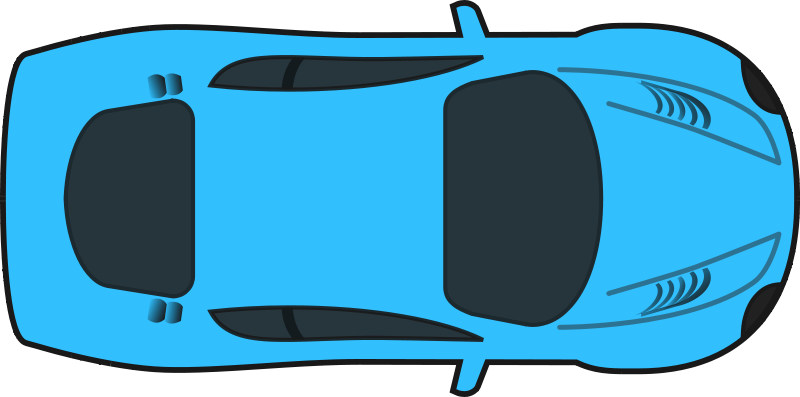
\includegraphics[width=0.7\linewidth]{../data/carClipArt.jpg}
                \caption{Model vozidla \cite{c:carmodel}} 
                \label{fig:carpic}
            \end{wrapfigure}

            Centrálním bodem celého projektu jsou závodnící ovládaní umělou intelignecí.
            Hlavním kritériem při jejich vývoji bylo předat sítím co největší kontrolu nad 
            vozidlem samotným. 

            \vspace{2em}
            \begin{figure}[H]
            \centering
            \begin{minipage}[t]{.5\textwidth}
                \centering
                \animategraphics[loop,autoplay,trim = 5.5cm 5.5cm 5.5cm 5.5cm,width=0.9\linewidth]{60}{data/forward/r_}{1}{60}
            \end{minipage}%
            \begin{minipage}[t]{.5\textwidth}
                \centering
                \animategraphics[loop,autoplay,trim = 5.5cm 5.5cm 5.5cm 5.5cm,width=0.9\linewidth]{60}{data/spin/r_}{1}{90}
            \end{minipage}
            \captionof{figure}{Povolená ovládání vozidel}
            \label{fig:controlls}
            \end{figure}

            Ovládání závodníkům dává plnou kontrolu nad \textbf{rychlostí a zatáčením s proměnlivou
            sílou otáčení}. S touto možností se závodnící při dostatečném tréninku zvládají naučit
            velmi optimalizované průjezdy závodními traťemi všeho druhu.

            \tab V architektuře neuronové sítě jsou do výstupní vrstvy zabudovány dva neurony.
            První určuje ovládání rychlosti a druhý zatáčení. Hodnoty, kterých na těchto neuronech
            může být dosaženo jsou upraveny do \textbf{rozsahu -1.0 - 1.0}. Tímto způsobem 
            má ovladač velkou kontrolu při rozhodování o síle zrychlení/zpomalení nebo o úhlu zatočení.

        \subsection{Kontrola prostředí}
            Aby se ovládání mohlo rozhodovat, je potřeba dodat data z prostředí kolem 
            jeho vozidla. Hlavním zdrojem informací (vstupní vrstva neuronové sítě) je \textbf{5
            dálkových senzorů}, které měří vzdálenost předního nárazníku od stěn před ním.
            Paprsky senzorů jsou vysílány z předního středového bodu vozidla bod zorným úhlem 
            120\textdegree{} s určitou maximální vzdáleností, které mohou dosáhnout. Poslední informací 
            je poté \textbf{interní časomíra vozidla}, která udává kolik proběhlo výpočtů od startu testu. 

            \vspace{1em}
            \begin{figure}[H]
            \centering
            \begin{minipage}[t]{.5\textwidth}
                \centering
                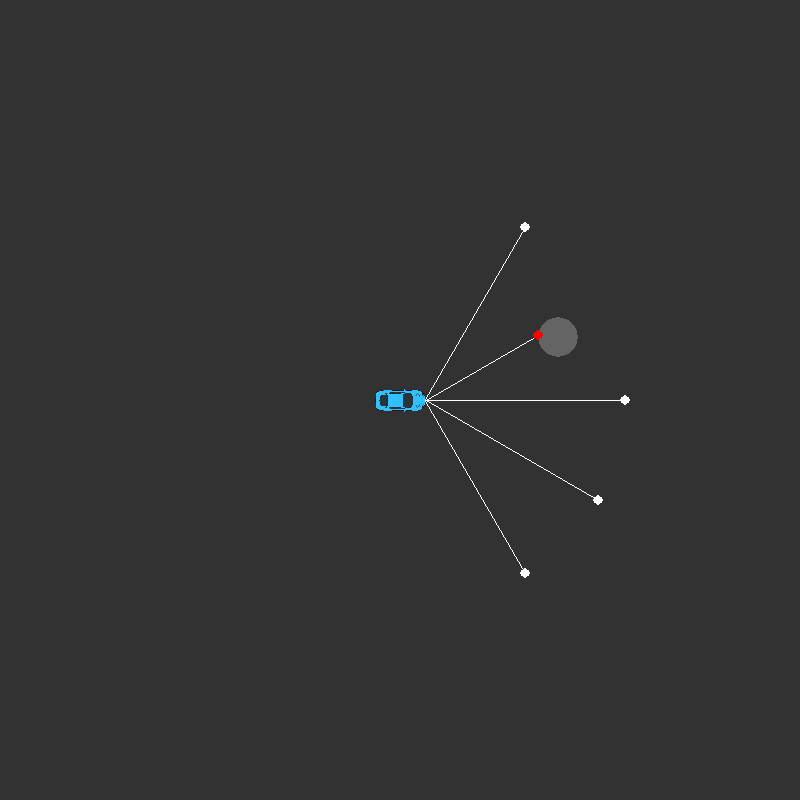
\includegraphics[trim = 5cm 5cm 5cm 5cm, clip, width=0.9\linewidth]{data/rays1.png}
                \caption*{Použité řešení}
            \end{minipage}%
            \begin{minipage}[t]{.5\textwidth}
                \centering
                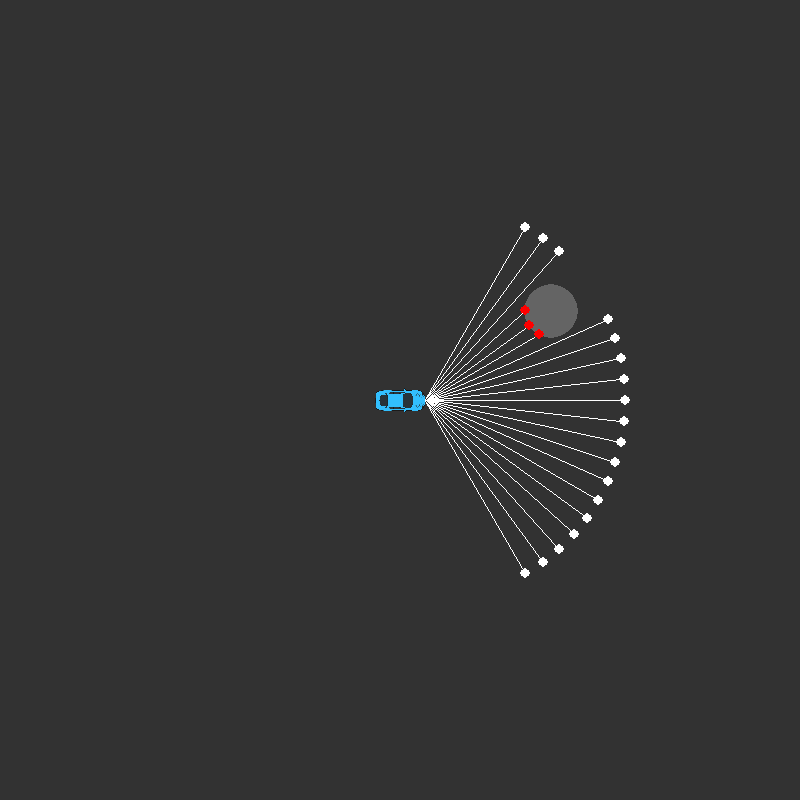
\includegraphics[trim = 5cm 5cm 5cm 5cm, clip, width=0.9\linewidth]{data/rays2.png}
                \caption*{Demonstrace paprsků}
            \end{minipage}
            \captionof{figure}{Práce měřících paprsků}
            \label{fig:rays}
            \end{figure}
            \pagebreak

            Vedle dálkových měřičů jsou ještě vozidla kontrolována proti kolizím s testovacím 
            prostředím. Případná kolize se stěnou závodní trati by ukončila testovací jízdu
            daného vozidla z generace a následně by byl vypočítán jeho výsledek (zdatnost).
            Tuto kontrolu zajišťuje \textbf{5 senzorů po obvodu modelu vozidla}. Kontrola
            kolize na nich probíhá každý výpočetní cyklus.
            \begin{figure}[H]
                \centering
                
\includegraphics[trim = 7cm 7cm 7cm 7cm, clip, width=0.4\textwidth]{data/collisionpoints.png}
                \captionof{figure}{Senzory kolize}
                \label{fig:collisionpoints}
            \end{figure}

        \vspace*{-3em}
        \subsection{Trénink}
            Před trénováním se musí vytvořit testovací prostředí (trať) a vložit
            do ní pár kontrolních bodů (START, ZÁCHYTNÉ BODY). Je potřeba zmínit,
            že každý trénink, i když bude prováděn na totožné trati, bude odlišný od těch
            předchozích. Příčinou je náhodnost celého procesu a styl jakým jsou vytvářeni
            náhodní jedinci pro první generaci testování.

            \tab Po nárazu všech závodníků nastává konec testování pro danou skupinu a 
            je vypočítána zdatnost každého z nich. Zde je potřeba určit \textbf{za co bude jedinec
            odměněn}. 
            
            \begin{center}
                \newcommand{\mr}[2]{
                    \multirow{#1}{*}{#2}
                }
                \vspace*{-1.5em}
                \hspace*{-4em}
                \begin{tabular}{ | c | c | c | c | p{8cm} | }
                    \hline
                    & Délka života & Počet z.b.* & Pořadí na z.b.* & Chování \\ \hline
                    \mr{2}{\textbf{Použito}} & \mr{2}{0,75 b.} & \mr{2}{50 b.} & \mr{2}{100 b.} & Rychlé učení celé trati, po dokončení 
                    snaha se na trati zrychlit.\\ \hline
                    & \mr{2}{1 b.} & \mr{2}{50 b.} & \mr{2}{25 b.} & Schopnost se trať naučit, pomalá jízda. Cena života větší než 
                    průjezd záchytnými body.\\ \hline
                    & \mr{3}{0,25 b.} & \mr{3}{50 b.} & \mr{3}{150 b.} & \textit{"Nastavení závodník"} - Velká rychlost na záchytných bodech.
                    Možné nevyřešení celé tratě. Délka života není tak cenná.\\
                \hline
                \end{tabular}
                \vspace*{-0.5em}
                \captionof*{table}{* z.b. = záchytný bod}
                \vspace*{-1em}
                \captionof{table}{Konfigurace odměn za výsledky na trati}
            \end{center}

            Po nalezení spráné konfigurace odměn a vyhovující architektury sítě
            se výsledky při opakovaném testování chovají vždy velmi podobně.
            Začátek je o pomalém postupu, kde se může vyskytnout jedinec, který
            je schopen se na trati dostat dál. Tento posun (\textbf{správná genetická informace})
            se rychle šíří i mezi zbytek populace. Poté nastává zlomový bod, kdy se
            v jedné generaci objeví takový jedinec, který je schopen projet trať celou
            (pouze primitivní "vyhýbání se stěnám", než optimalizovaný průjezd). 
            Tato informace se posléze začíná šířit i mezi ostatní jedince a začínají vznikat nové,
            lepší a rychlejší průjezdy. \textbf{V této fázi je problém (trať) vyřešen}.
            Toto řešení ale nemusí být to nejlepší, a tak i dále jde sledovat postupný nárůst
            úspěšnosti.\\
            Celý postup je na konci každé generace zaznamenáván do grafu.
            \begin{figure}[H]
                \centering
                \begin{minipage}[t]{.5\textwidth}
                    \centering
                    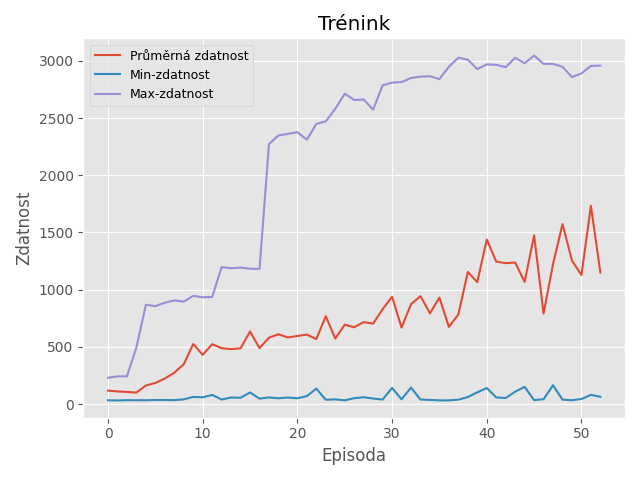
\includegraphics[trim = 0 1cm 0 1cm, clip, width=1\linewidth]{../data/f0.png}
                \end{minipage}%
                \begin{minipage}[t]{.5\textwidth}
                    \centering
                    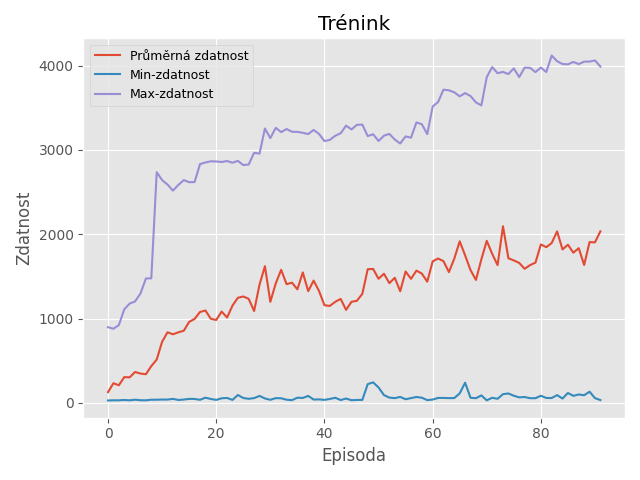
\includegraphics[trim = 0 1cm 0 1cm, clip,width=1\linewidth]{../data/f1.png}
                \end{minipage}
                \captionof{figure}{Výsledky tréninků na dvou různých tratích}
                \label{fig:results}
            \end{figure}

        \vspace{-2em}
        \subsection{Inteligence}
            \hfill
            \vspace{-2em}
            \begin{wrapfigure}[13]{r}{0.5\textwidth}
                \centering
                \animategraphics[loop,autoplay,width=0.8\linewidth]{24}{data/gif1/clever_anim-}{0}{158}
                \caption{Vychytralost} 
                \label{fig:intel}
            \end{wrapfigure}
            \\
            \tab Díky velkému množství různých možností, které se při učení vyzkouší, se ojediněle může stát,
            že jedinci naleznou a využijí \textbf{chyby v systému}(v testovacím prostředí). 
            I u mého programu se jedna taková chyba objevila a byla závodníky velmi rychle zneužita.\\
            Jednalo se o problém s průjezdem záchytným bodem, kdy zprvu v programu nebylo hlídáno, zda danný 
            bod byl již jedincem překonán nebo ne. To vedlo k rychlému zneužití, protože jak již bylo řečeno,
            za průjezd záchytným bodem se obrdží odměna. Toto byl velice rychlý a efektivní způsob zisku bodů.

    \section{Závěr}
        \tab I když se může zdát, že genetický algoritmus je plnohodnotnou variantou pro umělé inteligence
        a strojové učení, jedná se pouze o praktické uplatnění správné teorie, která je ale založena na spoustě náhodných procesů.
        Příroda tomuto postupu dává potřebný čas k nalezení téměř perfektních řešení každého problému.
        Ale v počítačové vědě, i když vše lze zvládat ve velké rychlosti, příroda má navrch.
        Proto existují různé systémy pro strojové učení, založené především na matematických postupech,
        které již náhodně nebádají po správném řešení, ale jdou cílevědomě přímo k němu.\\
        \tab Tento projekt může být pěknou ukázkou toho, jak jsou nové technologie přístupné pro veřejnost.
        O problematiku umělých inteligencí se zajímam již přibližně 3-4 roky. 
        Zájem o programování mi pak pomohl posunout tyto teoretické vědomosti do praxe skrz podobné programy.

    \bigskip
    \tableofcontents
    \listoffigures

    \begin{thebibliography}{6}
        \bibitem{c:perceptron}
            SAPORITO, G. What is a perceptron?. Perceptron model [online]. 2019 [cited 2020-06-10]. 
            Available from \url{https://miro.medium.com/max/1290/0*LJBO8UbtzK_SKMog}.

        \bibitem{c:easynn}
            NURAMI PUTRI, O. Titanic Prediction with Artificial Neural Network in R.. ANN model 
            [online]. 2018 [cited 2020-06-10]. Available from \url{https://cdn-images-1.medium.com/proxy/1*RGV6Bb3ChmVWsA8Q6Qth6Q.png}.

        \bibitem{c:relu}
            SARKAR, K. ReLU : Not a Differentiable Function: 
            Why used in Gradient Based Optimization? and Other Generalizations of ReLU.. [online]. 
            2018 [cited 2020-10-06]. Available from \url{https://medium.com/@kanchansarkar/relu-not-a-differentiable-function-why-used-in-gradient-based}\\\url{-optimization-7fef3a4cecec}.

        \bibitem{c:deepnn}
            BRE, F. Prediction of wind pressure coefficients on building surfaces using 
            Artificial Neural Networks. Artificial neural network architecture (ANN i-h 1-h 2-h n-o). 
            [online]. 2017 [cited 2020-06-10]. Available from \url{https://www.researchgate.net/profile/Facundo_Bre/publication/321259051/figure/fig1/AS:614329250496529@1523478915726/Artificial-neural-network-architecture-ANN-i-h-1-h-2-h-n-o.png}.

        \bibitem{c:crossover}
            KUMAR, A. Genetic Algorithms. Operators of Genetic Algorithms [online]. 2018 
            [cited 2020-06-10]. Available from \url{https://media.geeksforgeeks.org/wp-content/uploads/genetic-algorithm1.png}.

        \bibitem{c:carmodel}
            Clipart personal collection - Clipart Art [online]. 
            Dostupné z: \url{https://clipartart.com/images/car-clipart-sprite-sheet-3.jpg}

    \end{thebibliography}

    \vspace{2em}
    \begin{center}
        \footnotesize{
            \textbf{Vytvořeno v \LaTeX}
        }
    \end{center}
\end{document}
